
\section{Gen Strukturen}
\subsection{Struktur eines Prokaryotischen Gens}
\begin{itemize}
    \item Promotor
    \begin{itemize}
        \item Bindungstelle für \gls{Polymerase}
        \item Bindungstelle für Regulatoren (Repressor oder Aktivator)
    \end{itemize}
    \item Kodierende Region 
    \item \gls{Transcription terminator}
\end{itemize}
\begin{figure}[H]
    \centering 
     \begin{subfigure}[t]{0.8\textwidth}
    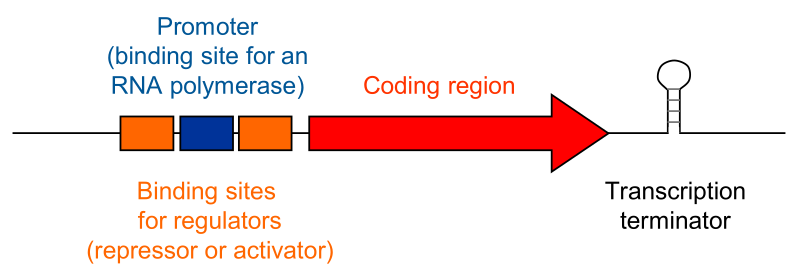
\includegraphics[width=\textwidth]{images/generalEukGene.png}
    \caption{General prokaryotic gene.}
    \label{fig:prokgene}
\end{subfigure}
    \begin{subfigure}[t]{0.8\textwidth}
    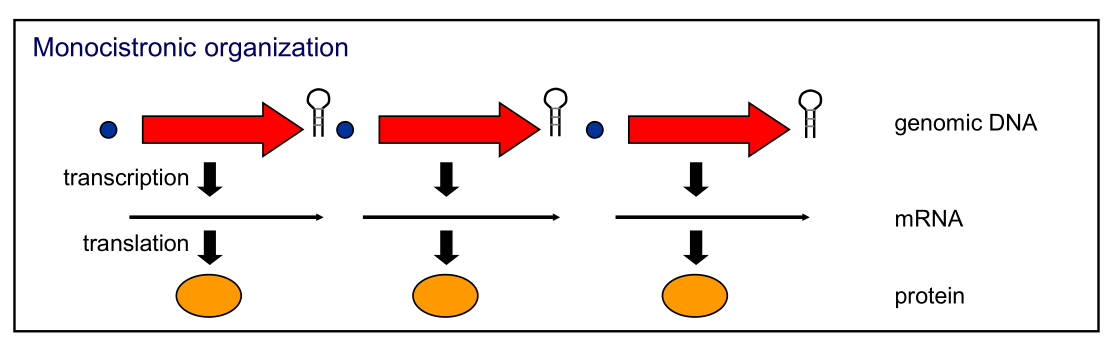
\includegraphics[width=\textwidth]{images/monocistronic.png}
    \caption{\index{Monocistronic}\textbf{Monocistronische Organisation.}
    Eine mRNA, die nur einen einzigen ORF (ein Gen) kodiert und damit nur ein Protein produziert. Typisch für Eukaryoten.}
    \label{fig:monocistronic}
\end{subfigure}
\begin{subfigure}[t]{0.8\textwidth}
    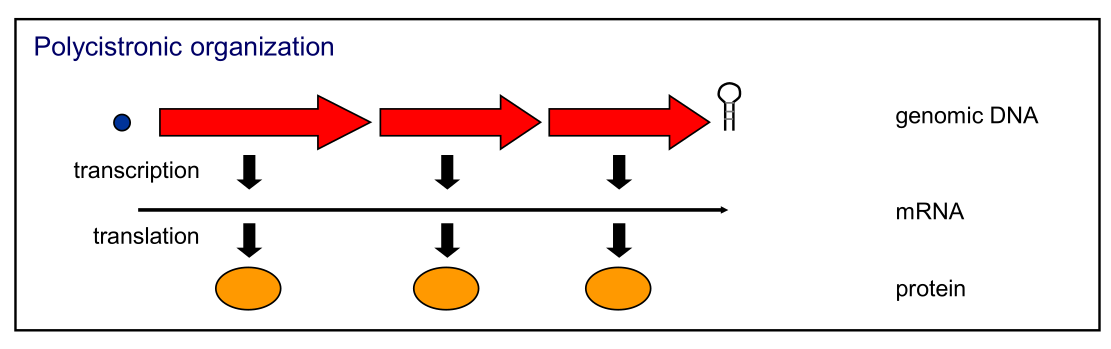
\includegraphics[width=\textwidth]{images/polycistronic.png}
    \caption{\index{Polycistronic} \textbf{Polycistronische Organisation.}
Eine mRNA, die mehrere \glspl{orf} hintereinander kodiert und mehrere Proteine werden von einer einzigen mRNA translatiert. Typisch für Prokaryoten (Operons). Jeder ORF hat eine eigene \gls{rbs}, aber es gibt einen gemeinsamen Terminator.}
    \label{fig:polycistronic}
\end{subfigure}
    \caption{Die zwei grundlegenden Modelle von prokaryotischen Genen.}
    \label{fig:cistronics}
\end{figure}

\subsection{Elemente eines Operons} \index{Operon}
\begin{figure}[H]
    \centering
    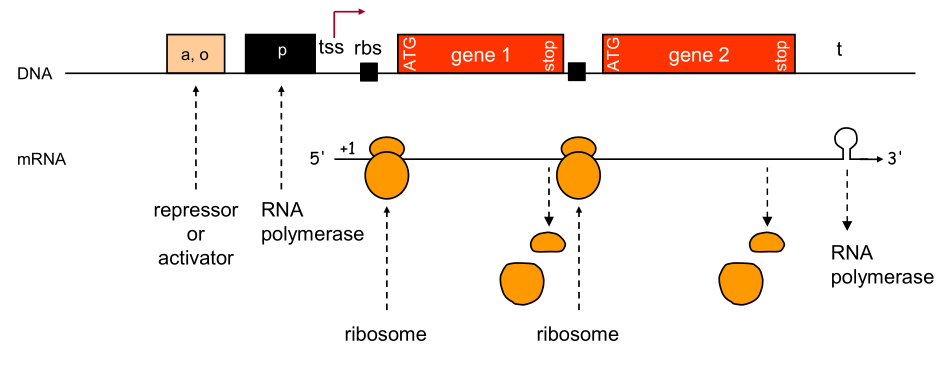
\includegraphics[width=0.8\linewidth]{images/operon.png}
    \caption{Aufbau und Elemente eines Operons}
    \label{fig:enter-label}
\end{figure}
\subsection{Translationelles Coupling}
Die Kopplung von Transkription und Translation ist ein Mechanismus der Genexpressionsregulation, bei dem die Synthese einer mRNA (Transkription) durch ihre gleichzeitige Entschlüsselung (Translation) beeinflusst wird. Bei Prokaryoten werden mRNAs bereits während ihrer Transkription translatiert. 
\subsection{Informationsfluss und Regulation in einer prokaryotischen Zelle}
Wichtig: Alle Level an Genexpression sind reguliert durch verschiedene Interaktionen: \begin{itemize}
    \item Protein-DNA
    \item Protein-RNA
    \item Protein-Protein
    \item DNA-RNA
    \item RNA-RNA
\end{itemize}
\section{Regulation der Genexpression} \index{Genexpression}
\index{Genexpression!Regulation der}
\subsection{Wichtige definitionen}
\begin{itemize}
    \item constitutive gene expression: \\ Nicht regulierte Genexpression, die kontinuierlich abläuft. 
    \item facultative gene expression:\\ Ein Gen wird nur transkribiert, wenn es benötigt wird.
    \item inducible gene expression:\\
    Ein Gen, dessen Expression auf ein Signal reagiert.
    \item positive regulation:\\
    Aktivierung oder Induktion der Genexpression.
    \item negative regulation: \\
    repression
    \item cis-acting element: \\ \index{cis-acting element}
    Regulatorisches Element, das physisch mit dem Gen verbunden ist, das es steuert.
    \item trans-acting element: \\ \index{trans-acting element}
    Regulatorisches Element, das nicht physisch mit dem Zielgen verbunden ist.
\end{itemize}
\begin{mybox}[title=Weitere Definitionen]
\paragraph{Apoaktivator:} Inaktive Form eines Aktivators – ohne gebundenen Liganden (Induktor) kann er nicht an die DNA binden und die Transkription nicht aktivieren. Erst Ligandenbindung erzeugt die aktive Konformation. Beispiel: CRP/CAP + cAMP im lac-Operon.
\paragraph{Aporepressor:} Inaktive Form eines Repressors – ohne gebundenen Corepressor kann er nicht an den Operator binden. Erst die Bindung des Corepressors (z.B. eines Metaboliten) erzeugt den aktiven Repressor → Genexpression wird abgeschaltet. Beispiel: Trp-Repressor + Tryptophan.
\end{mybox}
\subsection{Repression - Negative Genregulation} \index{Repression}
\begin{figure}[H]
    \centering
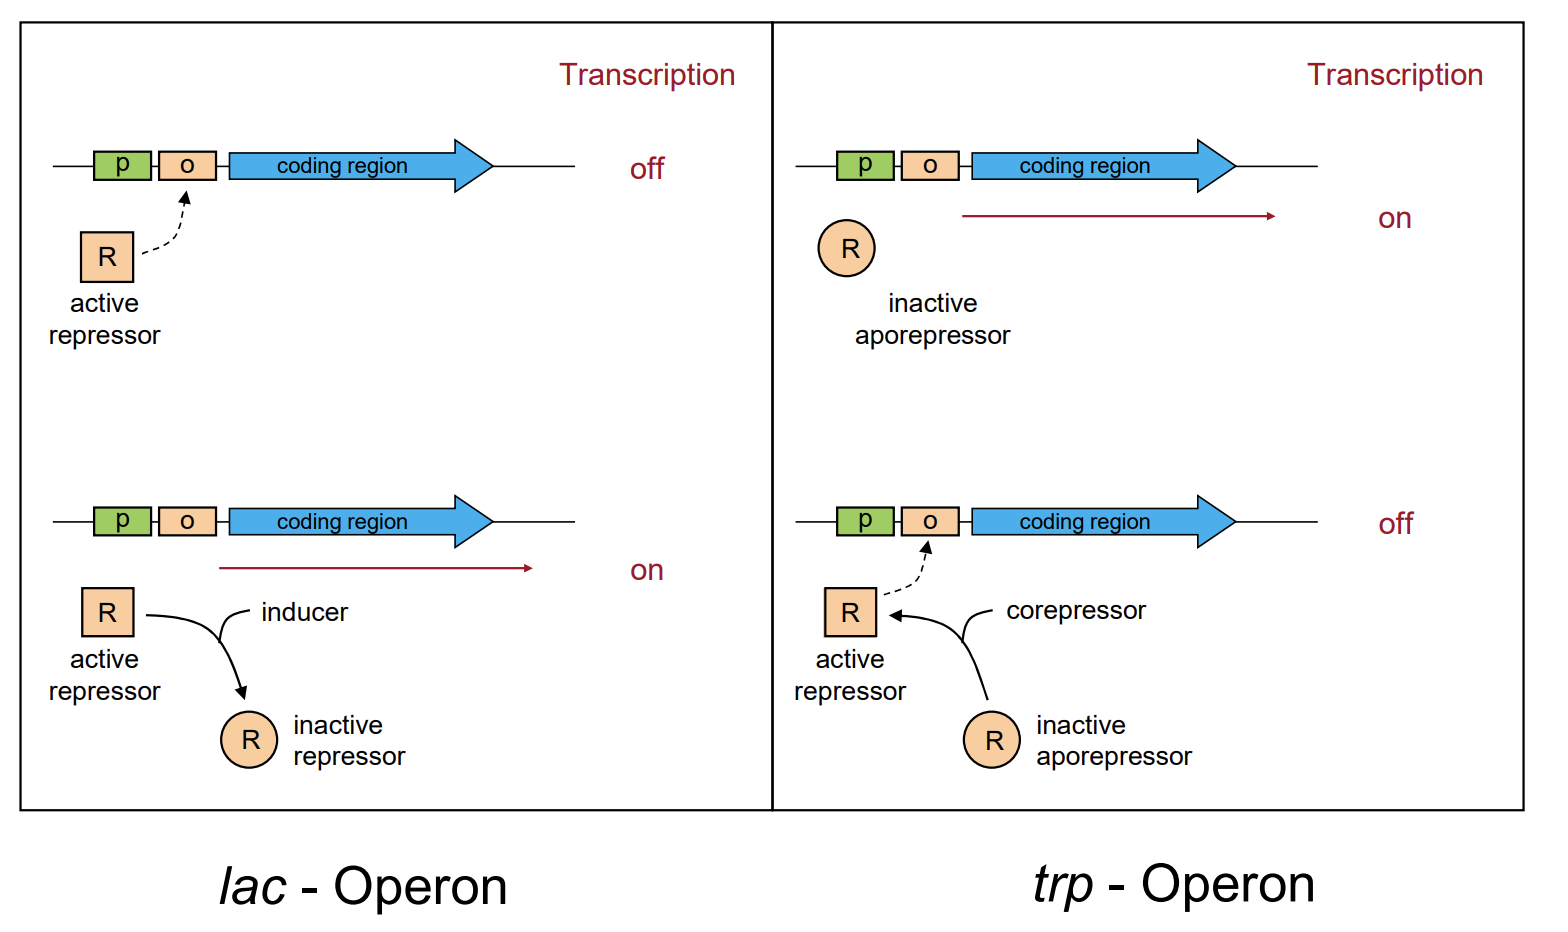
\includegraphics[width=0.8\linewidth]{images/Repression.png}
    \caption{Modell von Repressionen in Genexpressionen. Wichtig hierbei das binden an "O" und \gls{Inducer} und \gls{Corepressor}!}
    \label{fig:enter-label}
\end{figure}
\subsection{Activation - Positive Regulation der Genexpression}
\begin{figure}[H]
    \centering
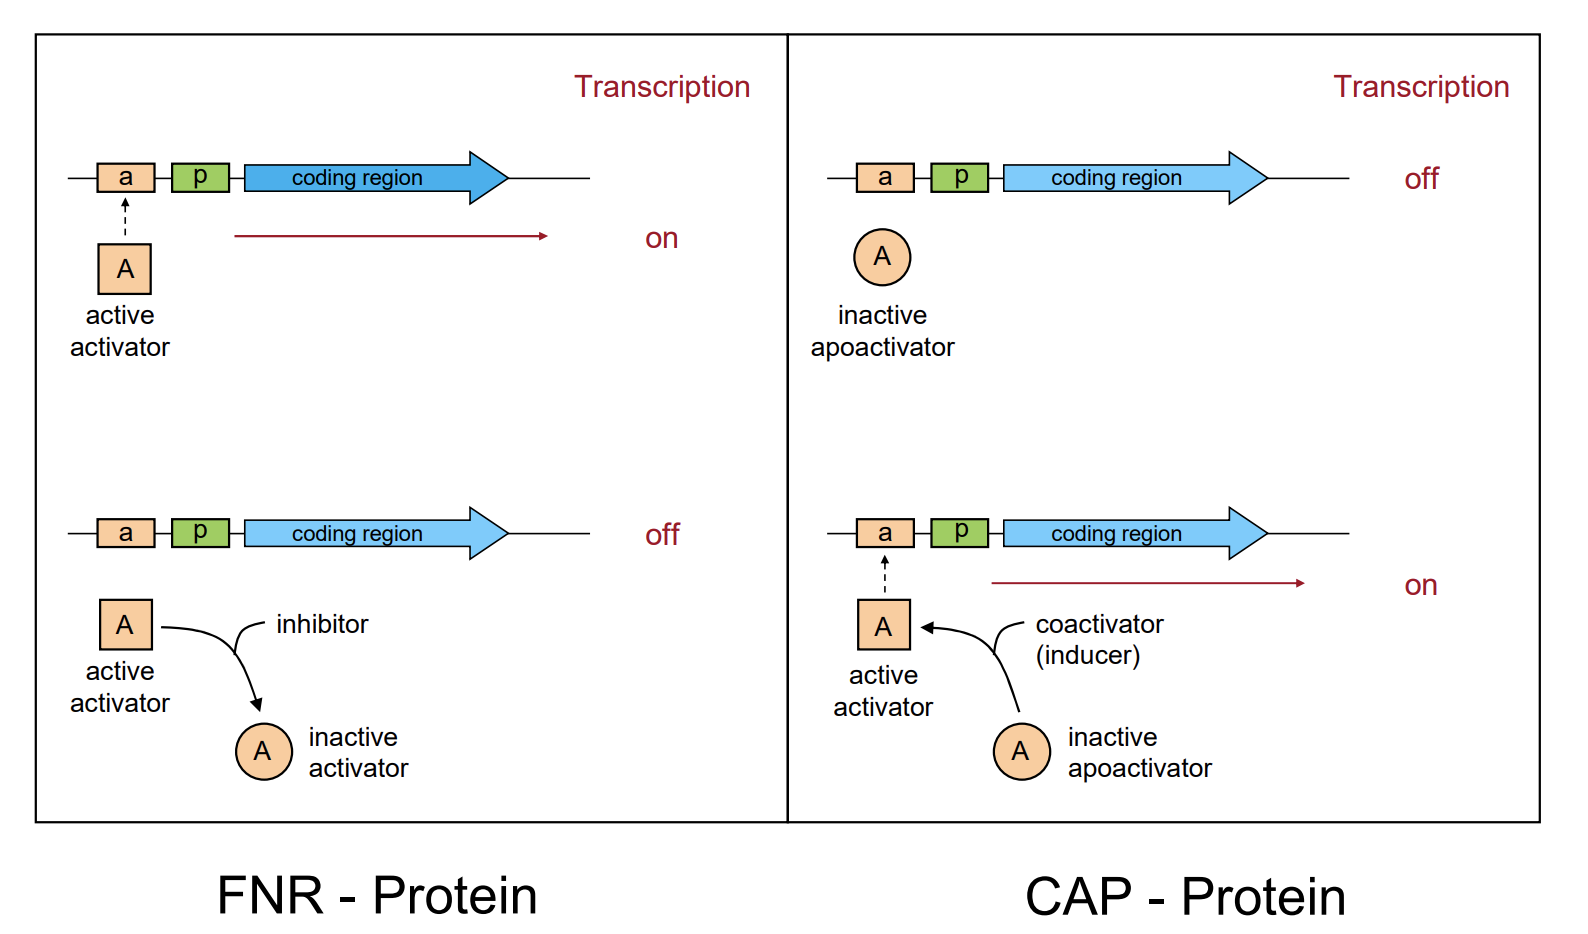
\includegraphics[width=0.8\linewidth]{images/Activator.png}
    \caption{Modell eines Aktivators. Wichtig hierbei das binden an Stelle "A" und inhibitor / coactivator}
    \label{fig:enter-label}
\end{figure}

\subsection{Definitionen}
\begin{itemize}
    \item \textbf{Modulon:} Eine Gruppe von Regulons oder Operons, die kollektiv auf Veränderungen der allgemeinen Bedingungen oder auf Stress reagieren, aber unter der Kontrolle unterschiedlicher oder sich überschneidender regulatorischer Moleküle stehen. \index{Modulon}
\end{itemize}
\begin{mechanism}[title= Definition Operon]\index{Operon}
Eine \gls{Transkriptionseinheit} mit Signalen für die RNA-Polymerase, um die Transkription zu starten und zu stoppen. Das Operon kann ein einzelnes Gen (monocistronisch) oder mehrere Gene (polycistronisch) enthalten. Gene werden durch ein polycistronisches Operon gemeinsam reguliert. \index{Operon}
\end{mechanism}
\begin{mechanism}[title= Definition Regulon]
Eine Gruppe von Operons, die sich über das gesamte Genom verteilen, aber von demselben Regulator gesteuert werden. \index{Regulon}

\end{mechanism}
\begin{mechanism}[title= Definition Stimulon]
Die Gesamtheit aller Operons, die auf denselben Stimulus reagieren. \index{Stimulon}
\end{mechanism}
\begin{mechanism}[title=Welche Rolle spielen die Transkriptionsfaktoren bei Operon\, Regulon u. Stimulon?]
Transkriptionsfaktoren binden an spezifische DNA-Sequenzen in der Nähe des Promotors eines Operons, um die Transkription der Gene zu regulieren. Sie können entweder als Aktivatoren wirken, die die Bindung der RNA-Polymerase fördern, oder als Repressoren, die die Transkription blockieren. Ein klassisches Beispiel ist das lac-Operon in E. coli, das durch den \textbf{lac-Repressor} reguliert wird. \\  \newline Ein \textbf{einzelner Transkriptionsfaktor} kann an die Promotorregionen \textbf{mehrerer Operons} oder Gene binden, um deren Expression in Reaktion auf bestimmte Signale zu koordinieren. \\ \newline \textbf{Mehrere Transkriptionsfaktoren }können beteiligt sein, um die Expression einer Vielzahl von Genen zu koordinieren, die auf den spezifischen \textbf{Stimulus} reagieren. 
\end{mechanism}
\index{Operon}
\section{Regulatorische RNAs in Bakterien}
Es gibt: 
\begin{itemize}
    \item Riboswitches \index{Riboswitch}
    \item \gls{srna} regulators
    \item CRISPR-Cas
\end{itemize}
\subsection{Riboswitches} \index{Riboswitch}
\begin{mechanism}[title=Definition Riboswitch]
Ein regulatorisches Segment einer mRNA, das direkt an ein kleines Molekül bindet und dadurch die Expression der kodierten Proteine beeinflusst.
\end{mechanism}\index{Riboswitch}
\begin{itemize}
    \item \textbf{Aptamer-Region:} Der Teil des Riboswitches, der das Molekül erkennt und bindet. \index{Aptamer-Region}
    \item \textbf{Expressionsplattform:} Der Teil, der strukturelle Änderungen durchführt, um die Genexpression zu regulieren. \index{Expressionsplattform}
    \begin{itemize}
        \item \textbf{Funktion:} Regulation der Transkription oder Translation in Abhängigkeit von Metaboliten.
    \end{itemize}
\end{itemize}
\begin{figure}[H]
    \centering
    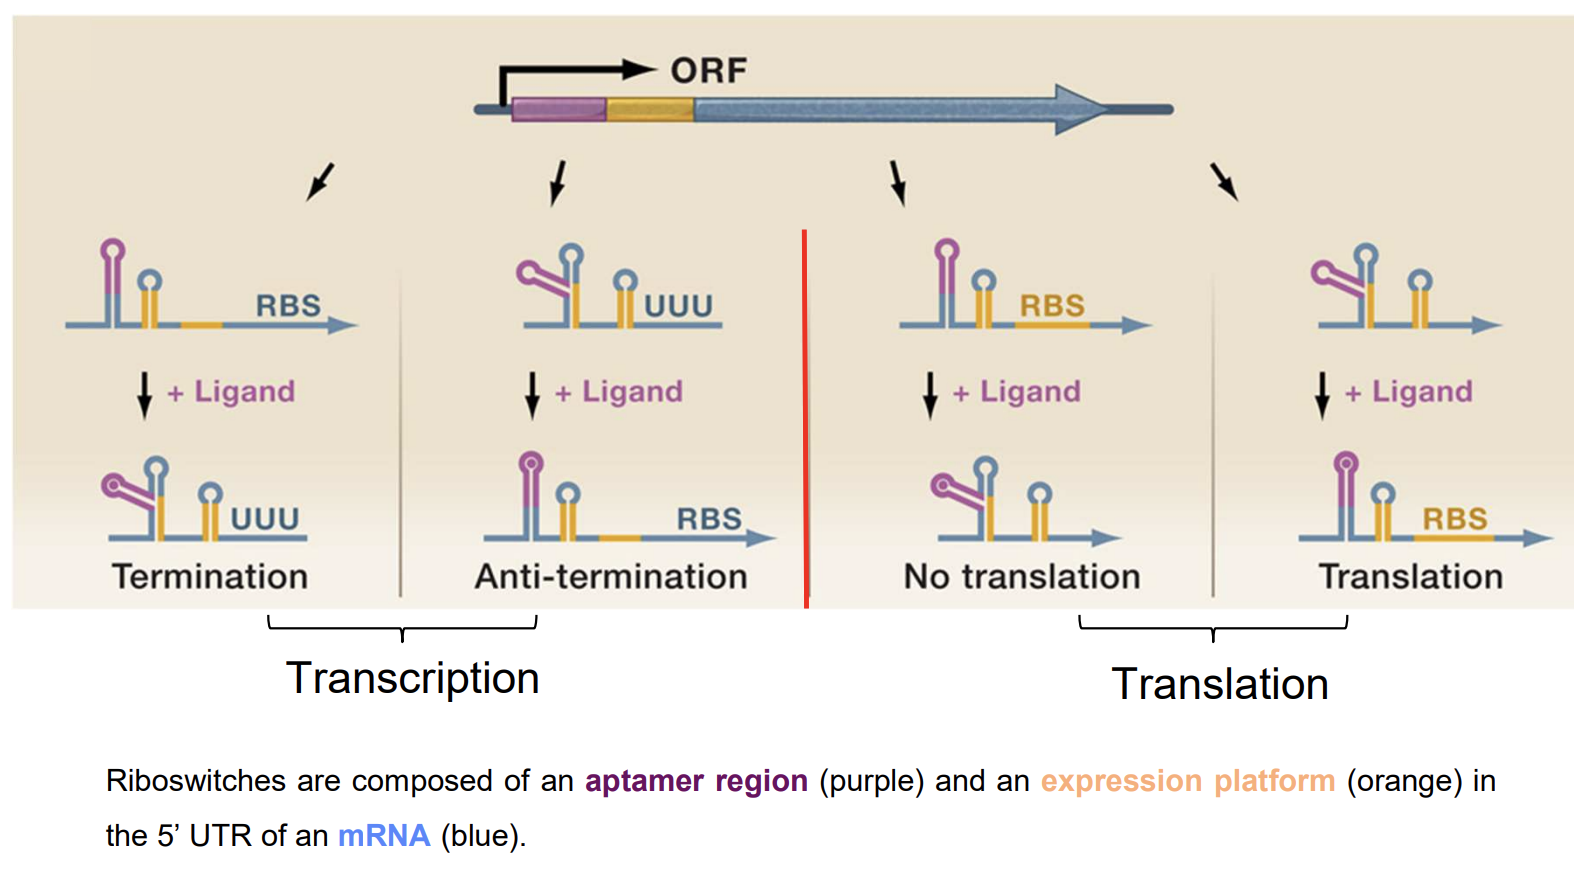
\includegraphics[width=0.8\linewidth]{images/Riboswitches.png}
    \label{fig:enter-label}
\end{figure}



\subsection{Aufbau eines RNA terminators}
\begin{figure}[H]
    \centering
    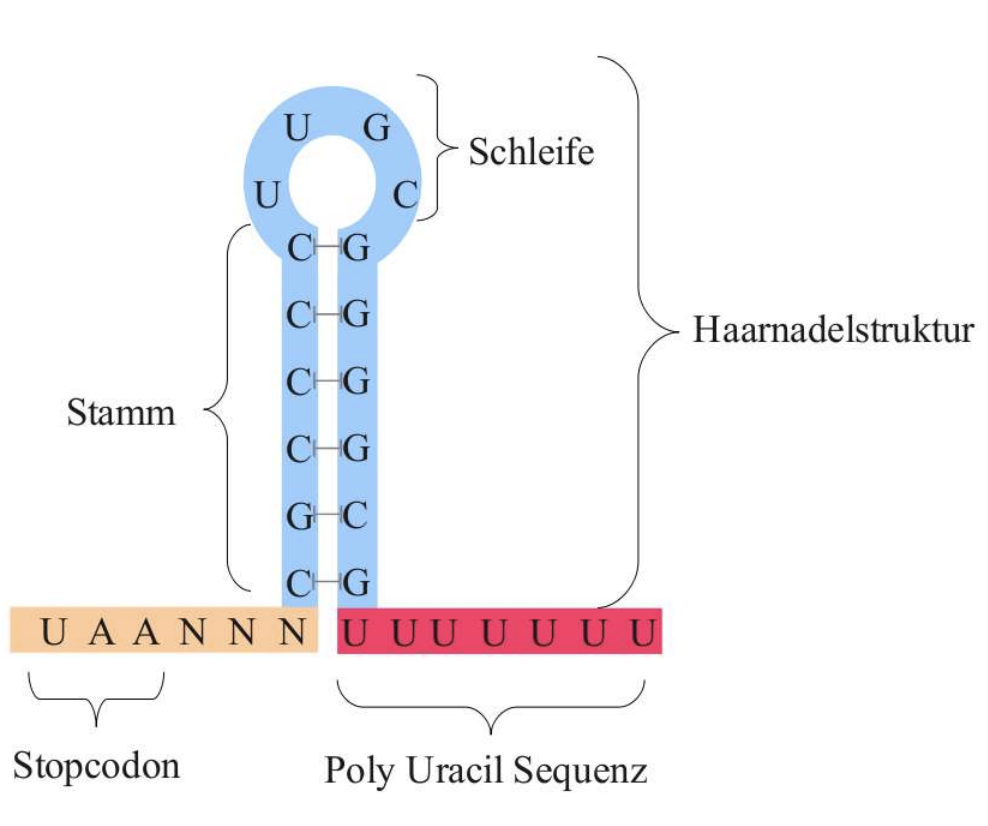
\includegraphics[width=0.5\linewidth]{images/Terminator.png}
    \caption{Abbildung eines Terminators }
    \label{fig:enter-label}
\end{figure}
\subsection{Small RNA (sRNA)}
\begin{itemize}
    \item \textbf{Small RNA (sRNA):} Kleine, nicht-kodierende RNA-Moleküle, die die Genexpression durch Basenpaarung mit mRNA regulieren.
    \item \textbf{Cis-kodierte sRNA:} Hat eine hohe Komplementarität zur Ziel-mRNA und wird am selben Genort transkribiert.
    \item \textbf{Trans-kodierte sRNA:} Hat eine begrenzte Komplementarität und wird von einem anderen Genort transkribiert.
    \item \textbf{Funktion:} Modulation der Translation, Stabilität und Abbau von mRNA. \index{RNA!sRNA}
\end{itemize}
\subsection{CRISPR-Cas-System} \index{CRISPR-Cas}
\begin{itemize}
    \item \textbf{CRISPR (Clustered Regularly Interspaced Short Palindromic Repeats):} Ein adaptives Immunsystem in Bakterien, das fremde DNA erkennt und zerschneidet.
    \item \textbf{Cas-Proteine:} CRISPR-assoziierte Proteine, die für den DNA-Schnitt verantwortlich sind.
    \item \textbf{crRNA (CRISPR RNA):} Führt die Erkennung der Ziel-DNA durch Basenpaarung.
    \item \textbf{tracrRNA:} Unterstützt die Reifung der crRNA und die Aktivierung des Cas9-Enzyms.
    \item \textbf{Cas9:} Eine Endonuklease, die doppelsträngige DNA an einer spezifischen Zielsequenz schneidet.
    \item \textbf{PAM (Protospacer Adjacent Motif):} Eine kurze DNA-Sequenz, die für die Erkennung durch Cas9 notwendig ist.
    \item \textbf{Anwendungen:} Genom-Editing, gezielte Genmodifikation, Krankheitstherapie und biotechnologische Forschung.
\end{itemize}
\subsubsection{Gene Drive}
Unter „Gene Drive“ versteht man Methoden zur Beschleunigung der Ausbreitung von Genen in Populationen.
\subsection{The RNA world hypothesis}
Riboswitches zeigen, dass natürlich vorkommende RNA kleine Moleküle spezifisch binden kann. Eine Fähigkeit, die viele bisher für eine Domäne der Proteine hielten.
Die Existenz von Riboswitches in allen Domänen des Lebens stützt daher die RNA-Welt-Hypothese, wonach das Leben ursprünglich ausschließlich auf RNA basierte und Proteine erst später hinzukamen.
Diese Hypothese setzt voraus, dass alle kritischen Funktionen, die von Proteinen ausgeführt werden (einschließlich der Bindung kleiner Moleküle), auch von RNA übernommen werden könnten.
Es wurde vermutet, dass einige Riboswitches möglicherweise uralte Regulationssysteme darstellen oder sogar Überreste von Ribozymen aus der RNA-Welt sind, deren Bindungsdomänen konserviert sind. 
\subsection{Sonstiges}
Random Info: Eukaryotic genes are usually longer than prokaryotic genes

\section{Splicing}
% Exon/Intron Boundaries nicht mit drin F 40
\subsection{Bildung einer mRNA bei Eukaryoten}
\begin{figure}[H]
    \centering
    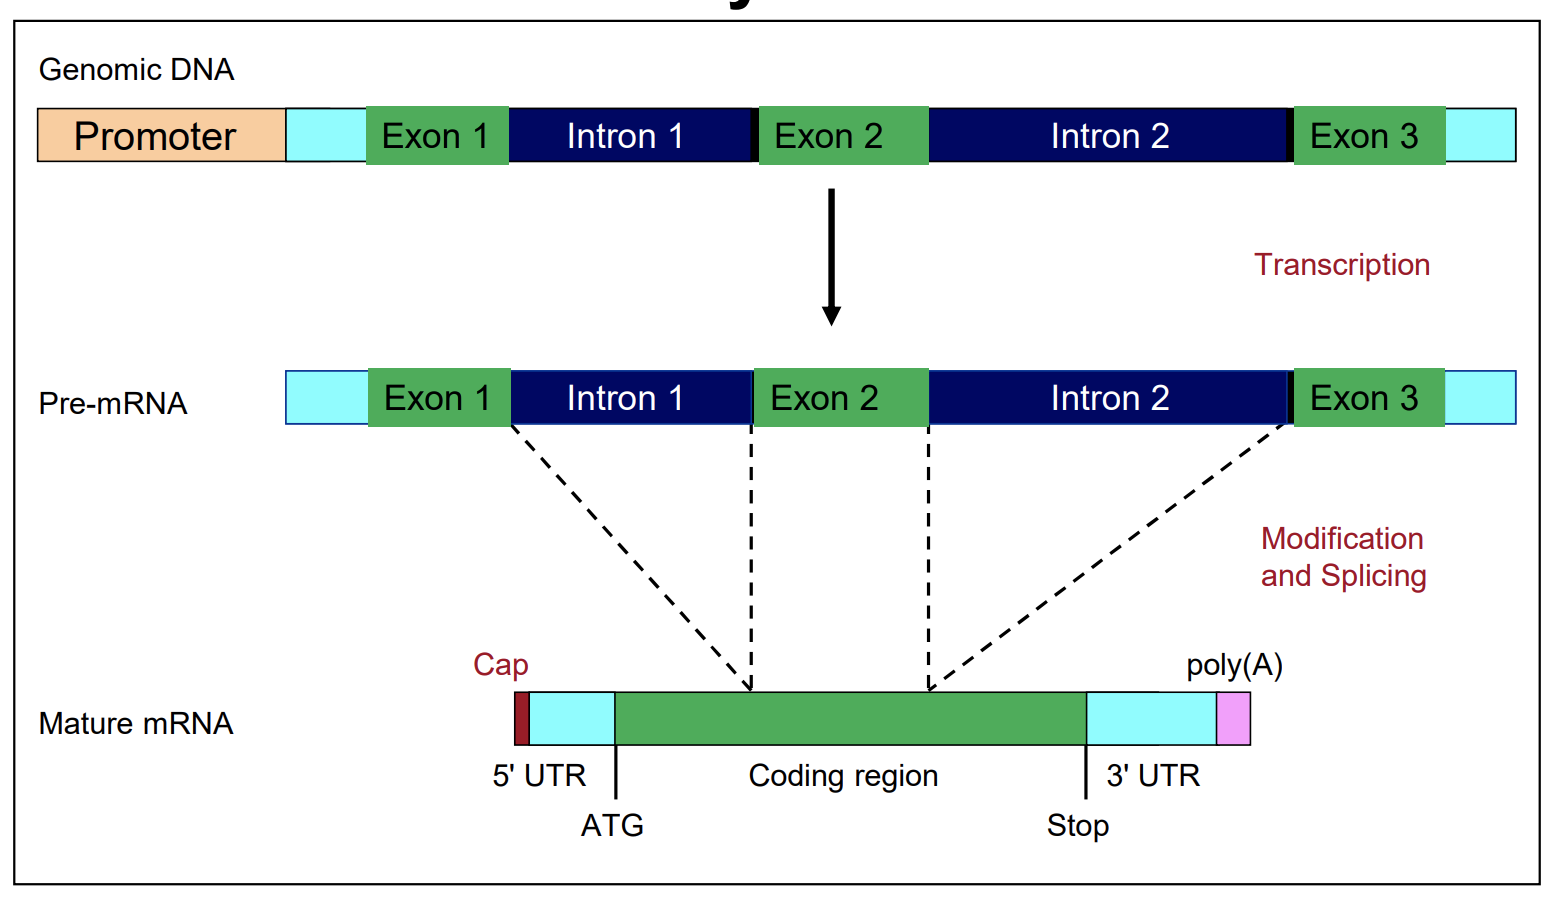
\includegraphics[width=0.8\linewidth]{images/mRNA.png}
    \caption{Verlauf des splicens (abstrakt).}
    \label{fig:enter-label}
\end{figure} \index{Splicing}


\begin{table}[H]
    \centering
    \begin{tabular}{p{7cm}p{1cm}p{7cm}}
        \textbf{Vorteile von Introns} & &\textbf{Nachteile von Introns} \\ \\
         Neue Kombinationen von Exons (Exon-Shuffling) können die Entstehung neuer Gene begünstigen, da Rekombinationen in neutralen DNA-Bereichen der Introns stattfinden können und funktionelle Domänen neu kombiniert werden können 
         & & Die Gen- und Genomgröße nimmt mit der Anzahl der Introns zu. Der Replikationsprozess benötigt mehr Zeit. Es ist ein genauer Mechanismus für die Entfernung der Introns aus der prä-mRNA erforderlich.
    \end{tabular}
\end{table}

\subsection{Typ von Introns} \index{Intron}
\subsubsection{Typ I}
Selbst-spleißend (Ribozym). Katalysieren ihre eigene Entfernung ohne Protein-Hilfe. Mechanismus: zwei Umesterungsreaktionen, initiiert durch ein freies Guanosin als Cofaktor. Vorkommen: Protozoen, Pilze, Chloroplasten, einige Bakteriophagen.
\subsubsection{Typ II}
Selbst-spleißend via Lariat-Intermediate (Schlaufe). Mechanismus ähnlich dem Spleißosom, evolutionär wahrscheinlich der Vorläufer. Vorkommen: Bakterien, Mitochondrien, Chloroplasten. Manche kodieren für eine Reverse Transkriptase und können als mobile Elemente agieren.
\begin{figure}[H]
    \centering
    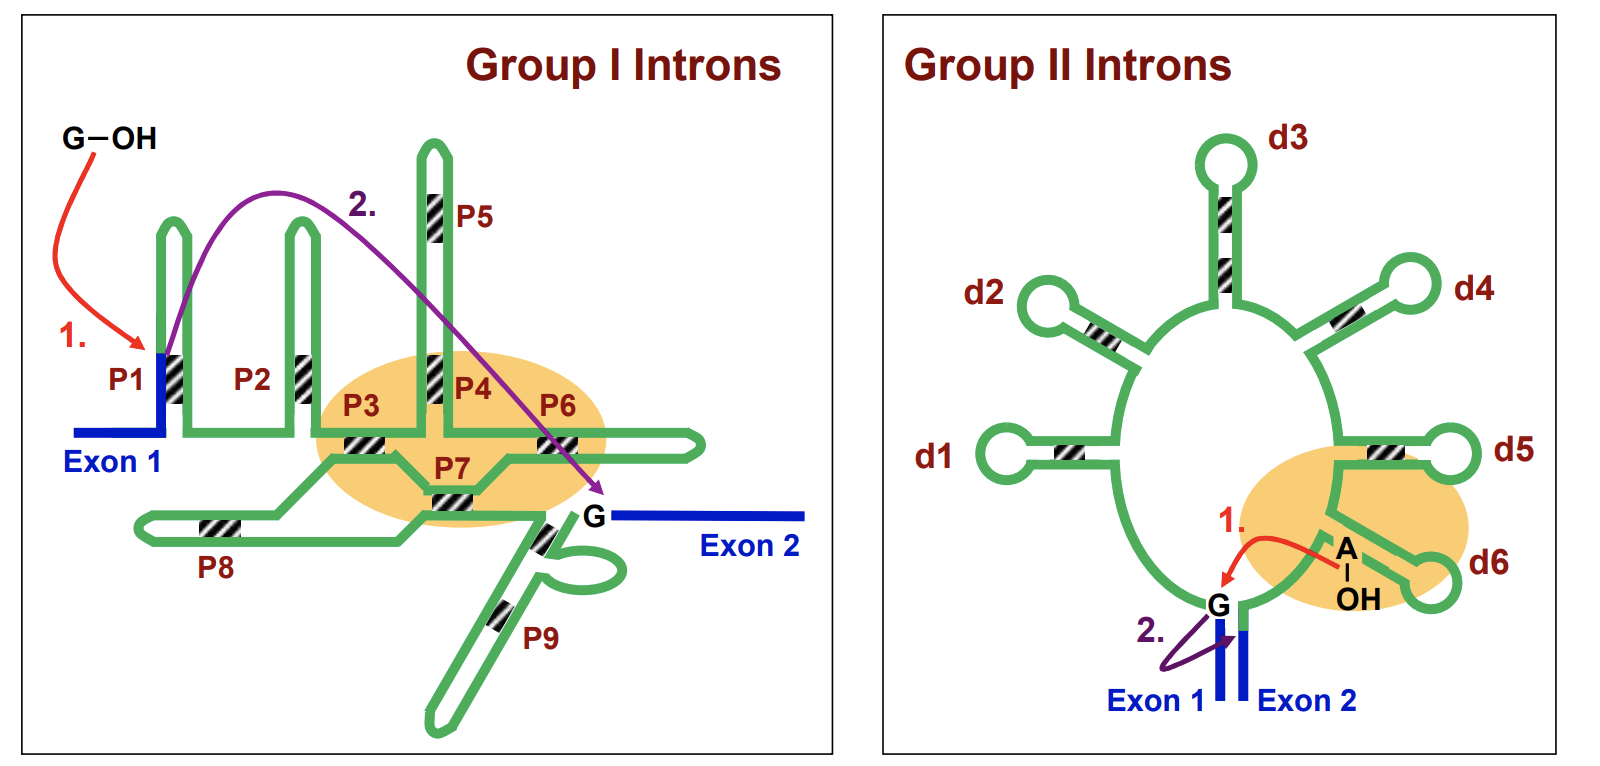
\includegraphics[width=0.8\linewidth]{images/IntronGruppen.png}
    \caption{Aufbau von den Introngruppen I und II. Der Strukturelle Unterschied zwischen beiden ist lediglich, dass Gruppe 1 die Exons an den Horizontalen Enden des komplexes hat. Gruppe 2 wiederum hat die Exon Abschnitte an den vertikalen enden.}
    \label{fig:enter-label}
\end{figure}

\subsubsection{Typ III - Spleißosom-abhängige Introns} Die häufigste Klasse in eukaryotischen Kerngenen. Werden durch das Spleißosom (Komplex aus snRNPs + Proteinen) entfernt.

\subsection{Alternatives Splicen} \index{Splicing!alternatives}
Verschiedene mRNA-Isoformen entstehen aus derselben prä-mRNA durch unterschiedliche Wahl der Spleißstellen. Mechanismen. Dies ermöglicht es aus einem Gen mehrere Proteinvarianten zu bilden und das ist wichtig für die proteomische Diversität 
% Typen von alternativem Spleißen
\begin{figure}[H]
    \centering
    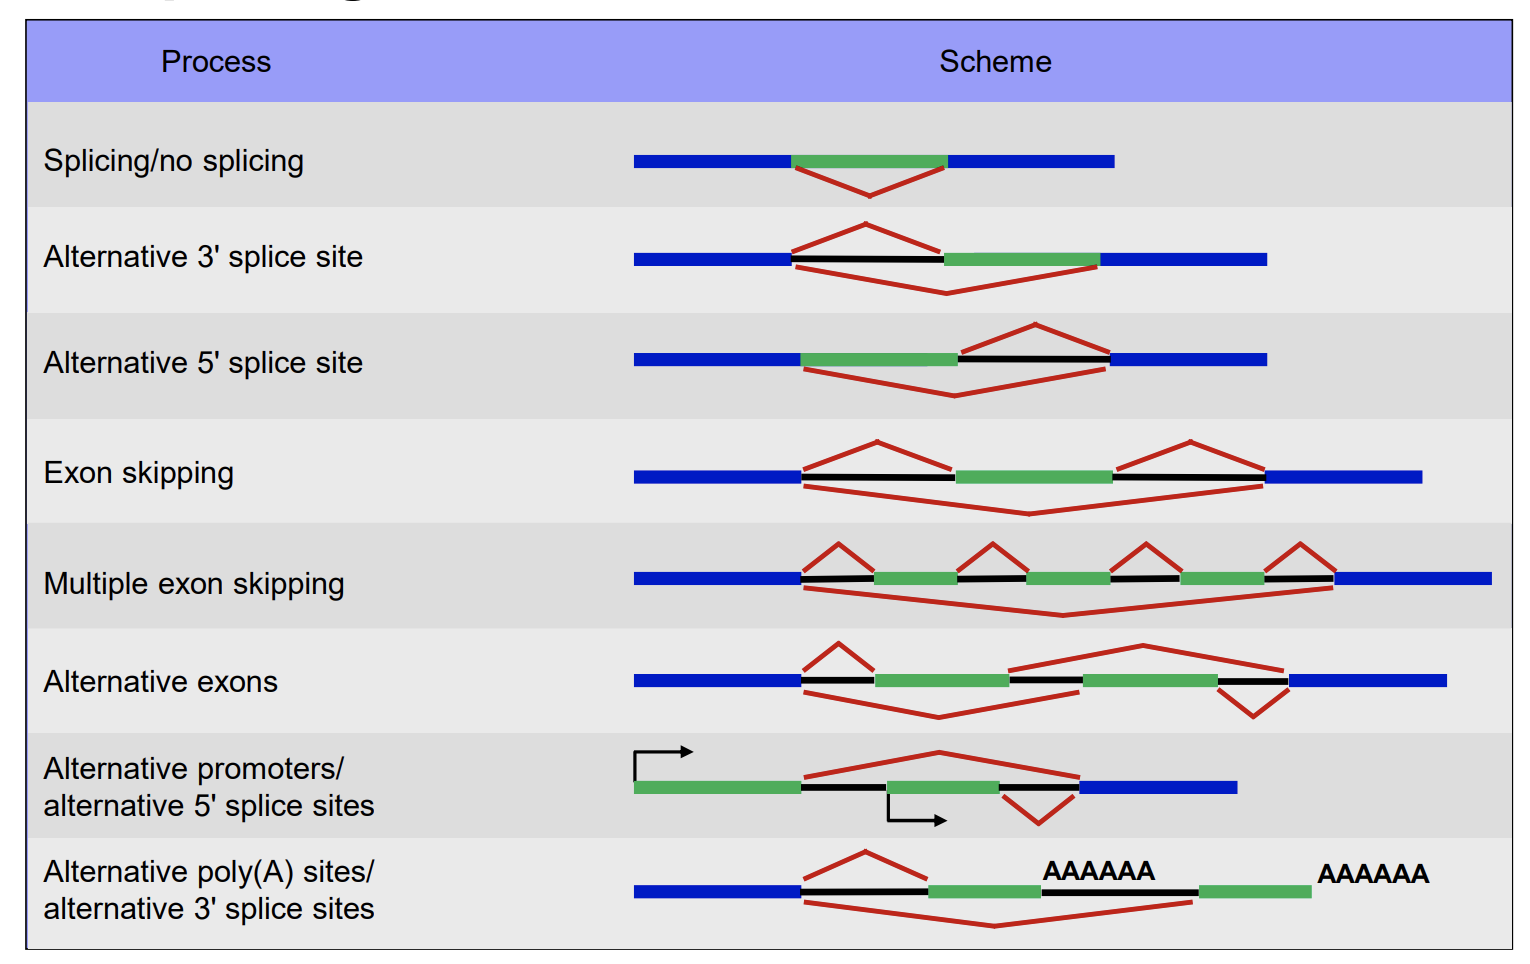
\includegraphics[width=0.8\linewidth]{images/Alternatives splicen.png}
    \caption{Verbildlichung der einzelnen Arten des alternativen splicens}
    \label{fig:enter-label}
\end{figure}

\subsection{Trans splicing}% F 43 
Spleißen zwischen Exons zweier verschiedener prä-mRNA-Moleküle (im Gegensatz zu normalem cis-Spleißen innerhalb einer mRNA). Ergebnis: chimäre mRNA aus Teilen zweier Gene. 

\section{RNA Editing}
RNA-Editierung ist ein molekularer Prozess, durch den einige Zellen diskrete Änderungen an spezifischen Nukleotidsequenzen innerhalb eines RNA-Moleküls vornehmen können, nachdem dieses von der RNA-\gls{Polymerase} erzeugt wurde.
\subsection{Insertion und deletion}
\begin{figure}[H]
    \centering
    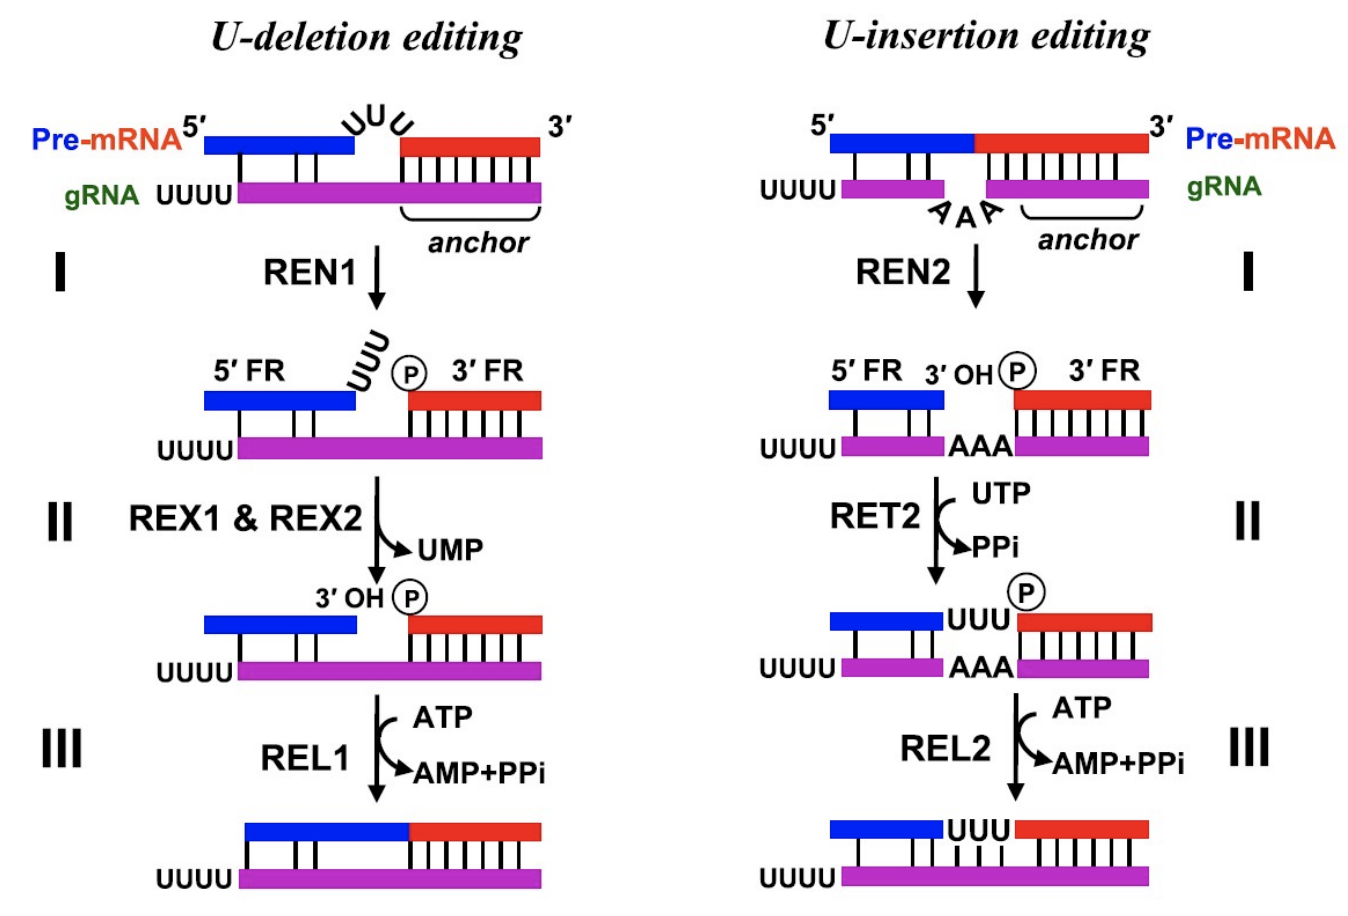
\includegraphics[width=0.8\linewidth]{images/Insertion und deletion.png}
    \label{fig:enter-label}
\end{figure}

\subsection{Deamination} %F 50 + 51
Grundlage des RNA-Editings: Enzymatische oder spontane Entfernung einer Aminogruppe von einer Base. 
\subsubsection{C zu U Editing}
Cytosin wird durch eine Desaminase enzymatisch zu Uracil konvertiert, ohne die DNA zu verändern. Beispiel: ApoB-mRNA im Darm – ein CAA-Codon (Glutamin) wird zu UAA (Stopp), also kürzeres ApoB-48 statt ApoB-100.
\subsubsection{A zu I Editing}
Adenosin wird durch ADAR-Enzyme (Adenosine Deaminases Acting on RNA) zu Inosin desaminiert. Inosin wird von der Translationsmaschinerie als Guanosin gelesen, es ist also effektiv eine A zu G-Änderung. Häufig in doppelsträngigen RNA-Strukturen. Beispiel: GluR-B-Rezeptor (Glutamatrezeptor), Änderung eines Codons beeinflusst Ionenkanal-Permeabilität.
\subsection{Risiken}
Mutationen in der RNA editing Maschinerie können zu schwerwiegenden Krankheiten führen wie: ALS, Epilepsie, Depressionen, Schizophränie, Prader-Willi Syndrom

\subsection{Amyotrophic Lateral Sclerosis}% F52
Bei ALS degeneriert eine bestimmte Untergruppe von Nervenzellen (Motoneuronen), was zu den mit ALS verbundenen fortschreitenden Symptomen führt: Muskelschwäche, Muskelschwund, Spastik und schließlich Lähmung und Atemversagen. \\
Die ungewöhnliche Asymmetrie der Motoneuronen mit Axonen von bis zu 1 Meter Länge macht sie besonders anfällig für Störungen des axonalen Transports und Stoffwechseldefekte.\\
Einer der vorgeschlagenen Mechanismen für den Nervenzelluntergang bei Patienten mit sporadischer ALS ist die AMPA-vermittelte Exzitotoxizität (der pathologische Prozess, bei dem Nervenzellen durch übermäßige Stimulation durch Neurotransmitter geschädigt oder abgetötet werden).

\section{Small regulatory RNA}
Kleine regulatorische RNAs sind nicht-kodierende RNA-Moleküle, die bei zellulären Prozessen wie der Aktivierung oder Hemmung eine Rolle spielen.  \\
Hauptklassen:
\begin{itemize}
    \item \gls{sirna}
    \item \gls{mirna}
    \item \gls{pirna}
\end{itemize}
%Ablauf als Bild dargestellt.
%\begin{figure}[H]
%    \centering
%    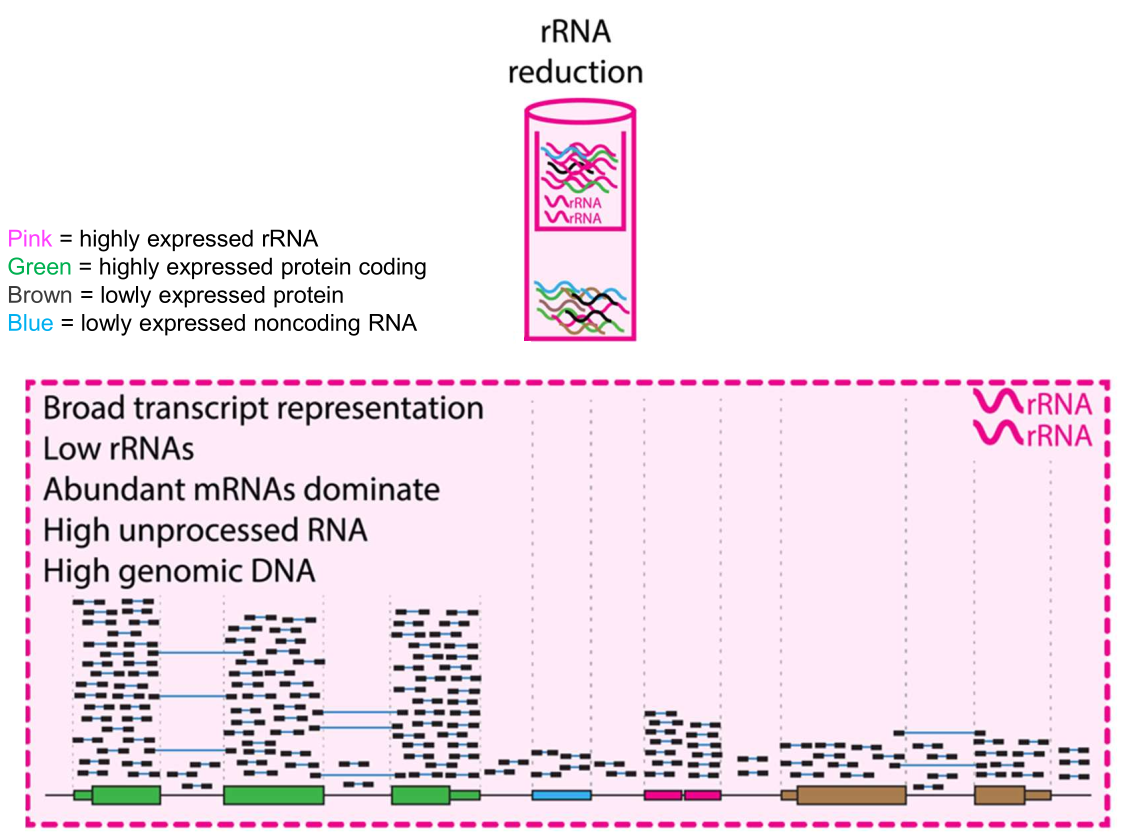
\includegraphics[width=0.8\linewidth]{images/rrna.png}
%    \label{fig:enter-label}
%\end{figure}
\subsection{siRNA Silencing} % F58
Small interfering RNAs werden durch Dicer aus langer dsRNA prozessiert. Der Antisense-Strang wird in den \gls{risc}-Komplex geladen. \gls{risc} bindet komplementär an Ziel-mRNA, die Ago2-Endonuklease schneidet die mRNA, es kommt zum Abbau und zum post-transkriptionellen Gensilencing. Hohe Sequenzspezifität; biotechnologisch als RNAi-Werkzeug genutzt. \\
Eine durch siRNA vermittelte Regulation kann zu Folgendem führen: 
\begin{itemize}
    \item Direktem mRNA-Abbau
    \item Translationshemmung und exonukleolytischem Abbau. 
    \item Heterochromatinbildung (bei Pflanzen führt die Bindung an das Zielmolekül zur Assoziation oder Aktivierung einer DNA-Methyltransferase (DMT), die die DNA methyliert, was zur Heterochromatinbildung führt). 
    \item Bei S. pombe und wahrscheinlich auch bei Tieren ist an diesem Signalweg eine Histon-Methyltransferase (HMT) beteiligt, die Lys9 des Histons H3 methyliert und dadurch die Heterochromatinisierung induziert.
\end{itemize}
\subsection{miRISC-Mediated Repression} % F59
Nicht unterdrückte mRNAs binden Initiationsfaktoren und ribosomale Untereinheiten an sich und bilden zirkularisierte Strukturen, die die Translation fördern. Wenn \glspl{mirisc} an mRNAs binden, können sie die Initiation im Stadium der Cap-Erkennung oder im Stadium der 60S-Rekrutierung unterdrücken. Alternativ können sie die Deadenylierung der mRNA induzieren und dadurch die Zirkularisierung der mRNA hemmen. Sie können auch eine Phase der Translation nach der Initiation unterdrücken, indem sie Ribosomen dazu veranlassen, vorzeitig abzuspringen. Schließlich können sie den Abbau der mRNA fördern, indem sie eine Deadenylierung gefolgt von einer Entkappung induzieren.
\subsection{Unequal cross-over}
\begin{mybox}[title=Definition unequal crossover]
Rekombinationsereignis zwischen nicht-homologen Positionen zweier Chromatiden, häufig durch Fehlpaarung repetitiver Sequenzen. \\
Ergebnis: ein Chromosom erhält eine Duplikation, das andere eine Deletion des betreffenden Abschnitts. Wichtiger Mechanismus für die Evolution von Genfamilien und für Copy Number Variations (CNVs). 
\end{mybox}
\begin{figure}[H]
    \centering
    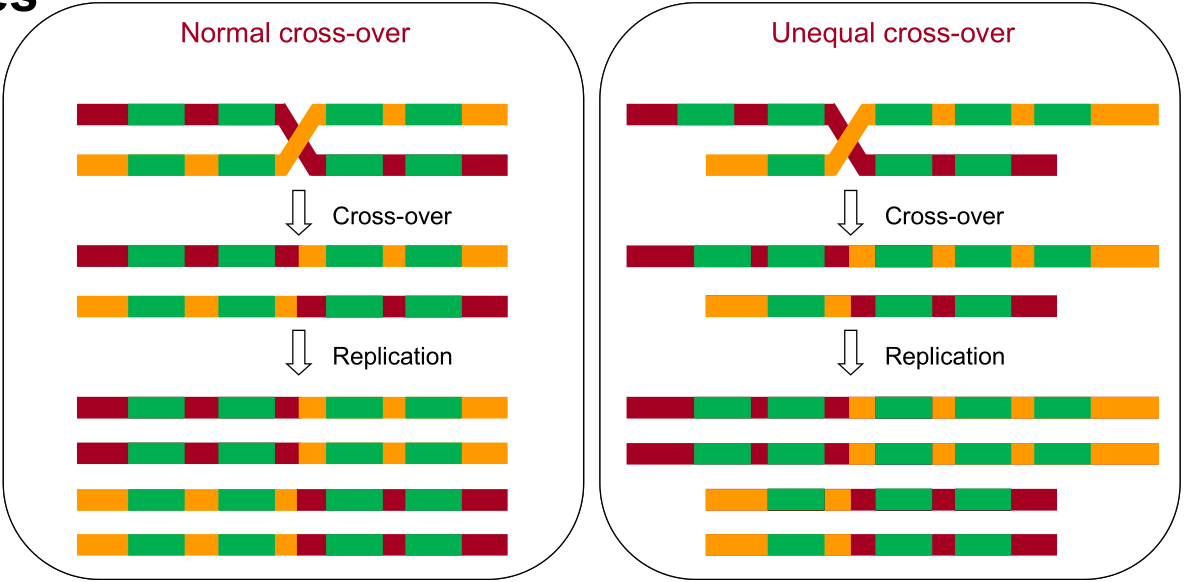
\includegraphics[width=0.8\linewidth]{images2/unequalcorssover.png}
    \caption{Unequal Crossover führt zu neuen Kombinationen von Genregionen.}
    \label{fig:my_label}
\end{figure}
\noindent Strukturelle und funktionelle Domänen von Proteinen werden häufig durch Exons kodiert. Es kann zu einer Neuanordnung von Exons und zur Entstehung von Genfamilien führen. 
\section{Genexpression Eukaryoten}
\subsection{Level der Regulation}
\begin{enumerate}
    \item Regulation der Transkription
    \item Regulation des Splicing
    \item Regulation des Transports aus dem Zellkern
    \item Degradierung der mRNA
    \item Translationale Regulation
    \item Proteinaktivität
\end{enumerate}
\subsection{Struktur}
\begin{figure}[H]
    \centering
     \begin{subfigure}[t]{0.8\textwidth}
    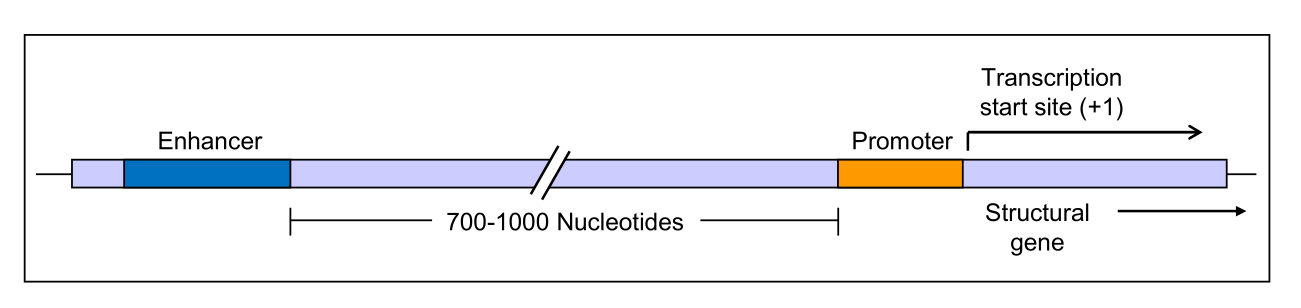
\includegraphics[width=\textwidth]{images/eukgengenerell.png}
    \caption{General eukaryotic gene. Die Promotorregion besteht aus modularen DNA-Sequenzen, die sich in der Regel 100 bis 110 Basenpaare stromaufwärts der Transkriptionsstartstelle befinden. \\
Neben den Promotorregionen wird die Transkription der meisten eukaryotischen Gene durch zusätzliche DNA-Sequenzen reguliert, die als Enhancer bezeichnet werden. \\
Die Position eines Enhancers muss nicht feststehen. Er kann sich stromaufwärts, stromabwärts oder innerhalb des Gens befinden, das er reguliert. Die Ausrichtung kann umgekehrt sein, ohne dass dies einen nennenswerten Einfluss auf seine Wirkung hat.}
    \label{fig:enter-label}
\end{subfigure}
 \begin{subfigure}[t]{0.8\textwidth}
    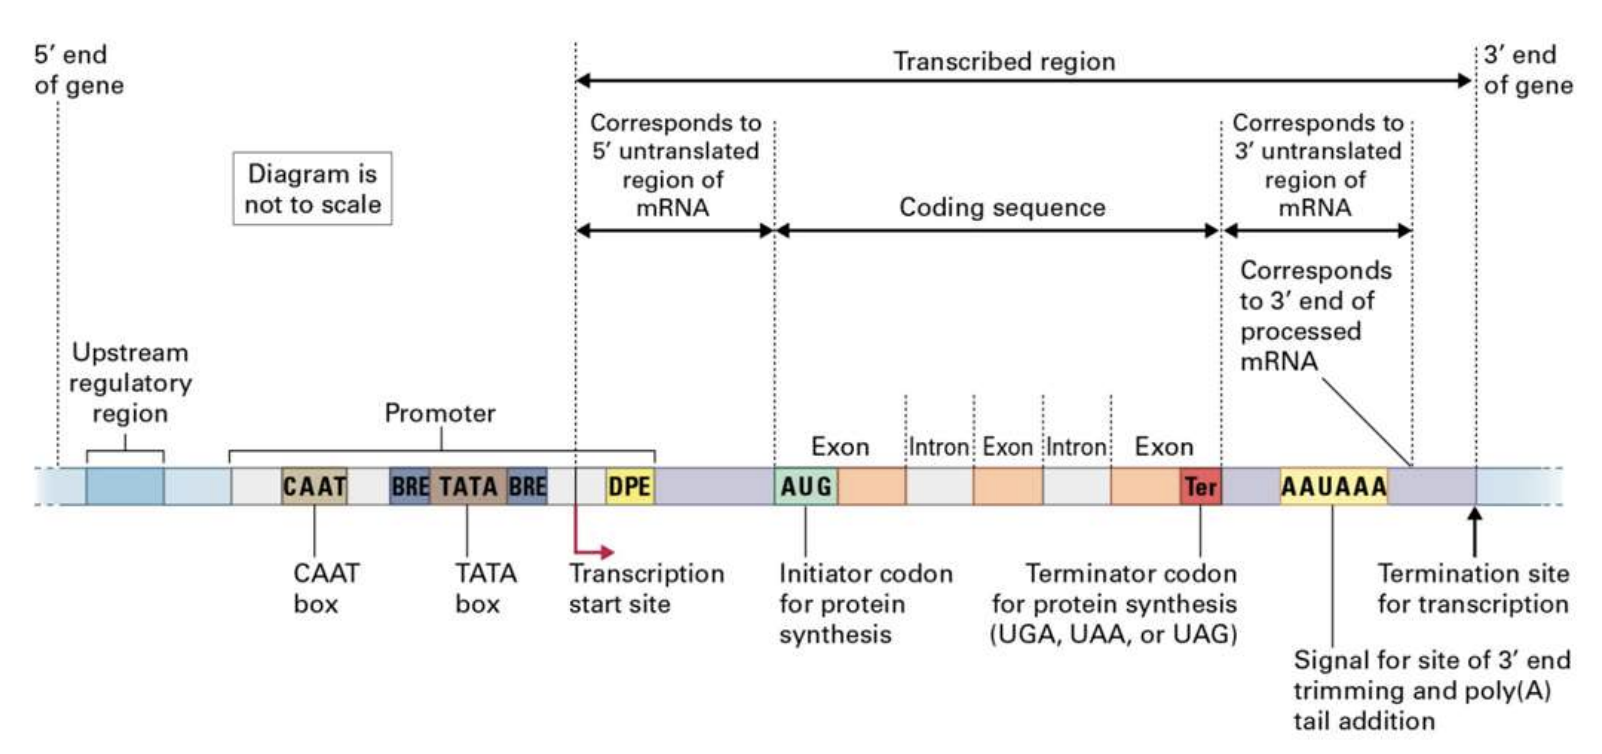
\includegraphics[width=\textwidth]{images/genexpression.png}
    \caption{Die Genexpression bei Eukaryoten weist mehrere einzigartige Merkmale auf und erfolgt stets über monozistronische Einheiten. }
    \label{fig:enter-label}
\end{subfigure}
  
\end{figure}
\begin{figure}[H]
    \centering
    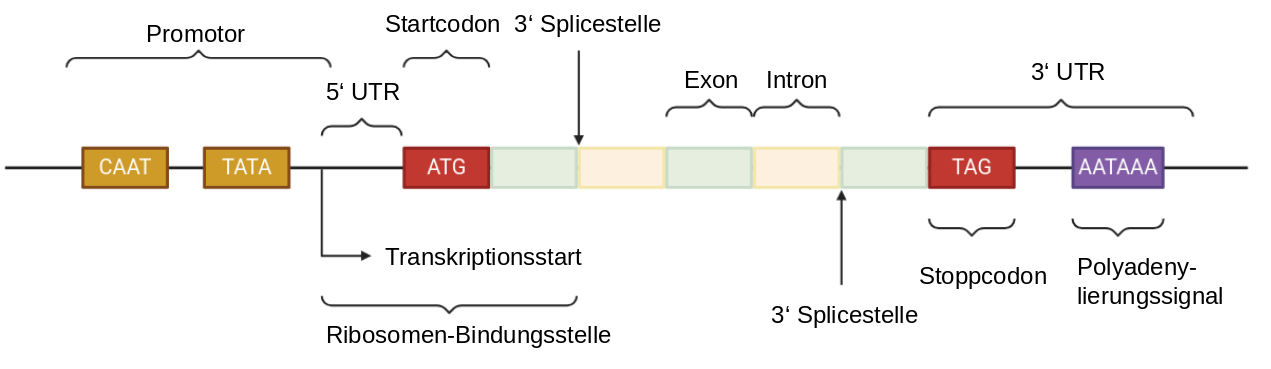
\includegraphics[width=0.8\linewidth]{images/eukgenfilled.png}
    \label{fig:eukgenfilled-label}
\end{figure}
